\documentclass{jflart}
\usepackage[utf8]{inputenc}
\usepackage[T1]{fontenc}
\usepackage{minted}

% Numéro et année des JFLAs visées par l'article, obligatoire.
\jfla{37}{2026}

\title{La programmation monadique dans le système de présentation Slipshow}
% Un titre plus court, optionnel.
%\titlerunning{Du bon usage de~\texttt{jflart.cls}}

% Auteurs, liste non abrégée.
\author{Paul-Elliot Anglès d'Auriac}
%% \author[2]{Cunégonde Martin}
%% \author[2]{Odoacre Contempierre}
% Une liste d'auteurs abrégée à utiliser à l'intérieur de l'article.
\authorrunning{Paul-Elliot}

% Affiliations des auteurs
%% \affil[1]{Université Paris Université, CNRS, INRIA, CEA, INRA, INSERM, Paris, 75013, France}
%% \affil[2]{Université Sorbonne Très Grand Sud, Nice, 06000, France}

% Une commande définie par l'utilisateur
%\newcommand{\cmd}[1]{\texttt{\textbackslash {#1}}}

\begin{document}

\maketitle

\begin{abstract}
  Slipshow est un logiciel de présentation, qui se focalise sur un style de
  discours plus ``continu'' que les slides. Très versatile, il permet à l'auteur
  de la présentations de déclencher de nombreuses actions à chaque étape, voire
  même d'en définir soi-même. Cela pose un défi ingénieural de taille : comment
  ``inverser'' l'execution d'une étape, quand le présentateur souhaite revenir
  en arrière ? Dans cet article, nous verrons la solution utilisée par Slipshow,
  basée sur le concept de Monades et son utilisation rendue aisée par le langage
  de programmation OCaml.
  %
  %% Il devrait contenir aussi peu de commandes LaTeX que possible pour faciliter
  %% la conversion vers HTML nécessaire à son inclusion dans les actes et sur le
  %% site web des JFLA.
\end{abstract}

\section{Introduction}

TODO: remplacer slide par ``diapositive''.

Slipshow est un logiciel de présentation, à l'instar de Beamer, Libre office
Impress ou Reveal.js. Il différe cependant fondamentalement de ces différents
exemples, en ce qu'il s'éloigne du concept de slides.

L'inspiration principale de Slipshow est la présentation au tableau. Celle-ci
est particulièrement adaptée aux sujets techniques et nécessitant un fort
support écrit pour aider la mémoire. Par exemple, lors d'un cours de
mathématique, il n'est pas rare de séparer le tableau en deux, et de n'effacer
qu'une moitié à la fois. Cela assure qu'au moins une moitié du contenu passé
sera accessible pour le public, en cas de distraction momentanée.

Au contraire, si une distraction intempestive survient peu avant le passage au
slide suivant, il est probable que le spectateur ait manqué une partie
importante de l'exposé, l'empêchant potentiellement de comprendre la suite.

Le concept de base d'une présentation Slipshow n'est pas le slide, mais le
``slip''. Conceptuellement, un slide est un carré de contenu, du même format que
l'écran le projetant. Un slip, lui, a la même largeur que l'écran, mais une
longueur arbitraire. Afin de montrer le contenu d'un slip, l'écran peut
``glisser'' pour en révéler les parties non visibles, à la manière d'un
navigateur permettant le déroulement d'une page web.

TODO: Figure.

\subsection{Contenu statique et dynamique}

Bien que les slips forment la génèse du projet Slipshow, celui-ci s'est bien
agrandi et supporte des présentations par slides, du style de Prezi, voire même
utilisant des animations tels que celles souvent utilisées dans les vidéos de
vulgarisation scientifique. En effet, une présentation Slipshow consiste en deux
parties entrelacées dans le fichier source:

\begin{itemize}
\item Une description du contenu statique : le texte, et sa mise en page définie de manière sémantique.
\item Une description de la dynamique de la présentation : l'ensemble des actions à effectuer, pour chaque étape.
\end{itemize}

Par exemple, considérons la présentation utilisant le système beamer suivante:

\definecolor{bg}{rgb}{.9, .9, .9}
\begin{minted}[bgcolor=bg]{latex}
  \begin{theorem}
    Ceci est un théorème
  \end{theorem}

  \pause

  \begin{itemize}
  \item premier point \pause
  \item deuxième point
  \end{itemize}
\end{minted}

correspondrait à la présentation Slipshow suivante:

\begin{minted}[bgcolor=bg]{markdown}
  {.theorem}
  Ceci est un théorème

  {pause}

  - premier point {pause}
  - deuxième point
\end{minted}


Hormis les différences de syntaxe, les deux versions se ressemblent beaucoup. Premièrement, le source de ces deux présentations est textuel, présentant un avantage par rapport à d'autres solutions tels Libreoffice Impress.

Le contenu statique est sous la forme de texte, utilisant une syntaxe spéciale\footnote{Syntaxe spéciale dont la définition ne sera pas l'objet de cet article. TODO: add link.} pour étiquetter des blocs d'une sémantique particulière (théorème, énumération), le système s'occupant de la mise en page à partir de ces étiquettes. Par exemple, l'environnement \verb|theorem| sera affiché différement d'une énumération à tirets.

Le contenu dynamique d'une présentation est ici défini dans le corps du texte, à nouveau à l'aide d'une syntaxe spéciale. Nous avons deux actions \verb|pause|, qui à leur activation révèlent le contenu qui suit. Ces actions sont définies dans le même flux que celui du texte.

Cependant, contrairement à $\LaTeX$/Beamer, l'ensemble des actions possibles pour Slipshow ne se limitent pas à \verb|pause|. En voici un petit aperçu:

\begin{itemize}
\item \verb|scroll-to=ID| déroule le slip courant jusqu'à ce que l'élément désigné soit entièrement visible.
\item \texttt{focus=ID} zoome sur l'élément désigné.
\item \verb|static=ID| insère un élément caché à sa position originelle.
\item \verb|play-media=ID| joue le fichier audio ou vidéo désginé.
\item \verb|speaker-notes| affiche des notes de présentateur dans la vue
  présentateur\footnote{Une fenêtre séparée, visible seulement par l'orateur,
    contenant un chronomètre et des notes.}.
\item \texttt{exec} exécute un script défini par l'utilisateur.
\end{itemize}


\subsection{Slipshow et le retour en arrière}

La compléxité du système d'actions de Slipshow pose un défi ingénieural de taille: comment gérer le retour en arrière? Lors d'une présentation, il est fréquent que l'orateur souhaite revenir à une étape précédente, par exemple pour clarifier un point ou répondre à une question.

Dans le cas de présentations classiques, le peu d'actions possibles (changer de slide, dissiper une pause) rend la définition d'un retour en arrière relativement simple. En effet, chaque action a une action inverse évidente: avancer d'un slide s'inverse en reculant d'un slide, dissiper une pause s'inverse en réappliquant la pause.

Dans le cas de Slipshow, la multiplicité des actions possibles, ainsi que leurs intéraction, rend la définition d'un retour en arrière plus ardue. Par exemple, l'action \verb|scroll-to=ID| n'a pas d'action inverse évidente: il faut se souvenir de la position de départ pour pouvoir y revenir. L'execution d'un script utilisateur peut modifier l'état de la présentation de manière arbitraire, rendant à priori impossible la définition d'une action inverse générique. Finalement, inverser de multiples actions exécutées successivement doit se faire dans un ordre précis, au risque de ne pas retrouver l'état initial.

Cette compléxité est purement en terme de lisibilité et maintenabilité du code, et non algorithmique. Il est facile de se rendre compte que théoriquement, l'on peut définir une fonction pour aller en avant dans la présentation, et une fonction pour retourner en arrière. Cependant, une manière naive de procéder risquerait d'être difficile à maintenir et à appréhender, avec une logique dupliquée et des risques d'incohérences.

Par exemple, lors de l'ajout d'une nouvelle action, il faudrait penser à ajouter son action inverse dans la fonction de retour en arrière. De plus, si une action est modifiée, il faudrait penser à modifier son action inverse en conséquence. Un système d'analyse statique serait difficile à mettre en place, on ne pourra donc compter que sur la vigilance du développeur.

Dans les toutes premières versions de Slipshow, le retour en arrière était implémenté à l'aide d'un système d'``instantanés''. Avant certaines actions, l'état courant de la présentation était stocké. Pour revenir en arrière, on revenait au dernier instantané, puis on repartait en avant jusqu'à l'étape précédente.

Cependant, cette méthode présentait de nombreux inconvénients, et était la source de nombreuses erreurs. L'impact mémoire était important, avec beaucoup de duplications d'état sauvegardés. Les nouvelles actions étaient difficile à rajouter, car leur fonctionnement interferait souvent avec le système d'instantanés. Par exemple, toute action ayant un effet d'animation impliquait un support spécial pour donner un effet de retour en arrière fluide.

La version 1.0 de Slipshow a constitué une réécriture complète du logiciel, dans le langage OCaml. Cette réécriture a été l'occasion de repenser le système de gestion du retour en arrière, et d'adopter une approche radicalement différente, basée sur la programmation monadique.

\subsection{Plan}

Dans cet article, nous commençons par définir ce qu'est une monade en
programmation, en prenant le langage de programmation OCaml pour les exemples.

Ensuite, nous montrons comment des monades ``classiques'' sont utilisées, en
particulier dans la base de code actuelle de Slipshow.

Nous terminons par la définition d'une monade originale, permettant de résoudre
élégament le problème initial du retour en arrière dans un outils de
présentation.

\section{Monades et programmation}

Les monades sont un concept issu de la théorie des catégories, popularisé dans le domaine de la programmation fonctionnelle par le langage Haskell.
Cependant leur utilisation en programmation et en théorie des catégories diffèrent. Dans cette dernière, une monade est un objet que l'on étudie pour ses propriétés mathématiques, propriétés que l'on démontre à l'aide de preuve rigoureuses.

En programmation, on utilise une ``monade'' comme un patron de conception, une manière d'organiser son code pour obtenir certains bénéfices. En particulier, les monades permettent d'encapsuler des effets de bord dans un programme fonctionnel, qui par nature n'en supporte pas.

Cependant, les qualités de ce patron de conception ne sont pas mesurable au sens mathématiques du terme. On peut seulement constater qu'il donne une manière uniforme d'exprimer de nombreux concepts, et qu'à un oeil habitué il rend leur manipulation plus aisé.

\subsection{Monades en théorie des catégories}

Si l'objectif de cet article n'est pas de s'étendre sur la théorie des catégories, il est intéressant de comprendre d'où la terminologie des ``monades'' vient.

\begin{defi}[Monade]
  Blablabla
\end{defi}

\subsection{Les monades en OCaml}

Dans cette section, nous allons voir une présentation accelérée du patron de
conception des monades. Nous allons découper cette explication en trois parties,
correspondant à des notions classiques de plus en plus proches des monades : les
``foncteurs'', les ``applicatifs'' et les monades elles-même.

Les monades permettent de faire des calculs avec, non des valeurs, mais des valeurs \texttt{spéciales}, tout en faisant comme-ci c'étaient des valeurs normales. La notion de spéciale sera à préciser, mais prenons tout de suite un exemple : les valeurs dont le calcul a produit une (ou plusieurs) erreurs.

\begin{minted}{ocaml}
type erreur = string

type 'a t = Ok of 'a | Error of erreur list
\end{minted}

Les monades promettent de pouvoir calculer avec ces valeurs ``spéciales'', comme
si elles étaient de valeurs normales. Pour cela, nous allons voir comment ``réifier'' des calculs de type \texttt{'a -> 'b} en des calculs de type \texttt{'a t -> 'b t}.

\subsubsection{Les foncteurs}

\begin{defi}[Foncteur]
  Un foncteur (au sens du patron de conception, pas des foncteurs de modules
  OCaml) est un type paramétré \texttt{'a t} et une fonction \texttt{map}:

  \begin{minted}{ocaml}
  type 'a t = ...

  val map : ('a -> 'b) -> ('a t -> 'b t)
  \end{minted}

  Qui soit tel que si \texttt{f : 'a -> b} et \texttt{g : 'b -> 'c}, et
  \texttt{(o)} est la composition de fonction, alors les fonctions \texttt{map (g o f)} et \texttt{(map
    g) o (map f)} coincident.
\end{defi}

La fonction \texttt{map} ``réifie'' un calcul de valeur normales, en un calcul
de valeurs spéciales. La condition supplémentaire assure que les réifications
sont sensées : calculer dans les valeurs spéciales est bien compatible avec le
calcul dans les valeurs normales. Dans notre exemple de valeurs qui peuvent être
des erreurs, nous pouvons définir une telle fonction de réification:

\begin{minted}{ocaml}
let map f = function
  | Ok x -> Ok (f x)
  | Error _ as x -> x
\end{minted}

Si les foncteurs permettent de réifier un calcul représenté par une fonction à une variable, ils sont cependant rapidement limités : leur définition est trop générale pour permettre de réifier des fonctions à multiples arguments, sous formes curryfiées. En effet, étant donnée une fonction \texttt{'a -> 'b -> c}, on peut grâce à \texttt{map} obtenir une fonction de la forme \texttt{'a t -> ('b -> 'c) t}, et non ce que l'on souhaiterait : \texttt{'a t -> 'b t -> 'c t}.

\subsubsection{Les applicatifs}

\begin{defi}[Applicatif]
  Un foncteur applicatif est un foncteur \texttt{'a t, map : ('a -> 'b) -> ('a t -> 'b t)} muni de deux fonctions supplémentaires:

  \begin{minted}{ocaml}
  val pure : 'a -> 'a t
  val app : ('a -> 'b) t -> ('a t -> 'b t)
  \end{minted}

  Qui soit tel que TODO.
\end{defi}

Notons que l'on est maintenant capable de réifier une fonction à deux variables
: si \texttt{f} st de type \texttt{'a -> 'b -> 'c}, alors \texttt{map f : 'a t
  -> ('b -> 'c) t}. Et donc \texttt{fun x -> app (map f x) : 'a t -> 'b t -> 'c
  t}.

Reprenant notre exemple des valeurs à erreurs, nous pouvons l'étendre en un foncteur applicatif :

\begin{minted}{ocaml}
let pure x = Ok x
let app f x = match f, x with
  | Ok f, Ok x -> Ok (f x)
  | Error x, Error y -> Error (x @ y)
  | (Error _ as err), Ok _ | Ok _, (Error _ as err)
     -> err
\end{minted}

Notons ici que nous avons défini un moyen de combiner deux valeurs spéciales : \texttt{f} et \texttt{x}. C'est en effet l'essence d'un applicatif : la combinaison de deux valeurs spéciales en une, afin de pouvoir continuer notre calcul avec les deux valeurs. En effet, nous pouvons remplacer, dans la définition d'un foncteur applicatif, la fonction \texttt{app} par la fonction \texttt{pair} suivante:

\begin{minted}{ocaml}
val pair : 'a t -> 'b t -> ('a * 'b) t
\end{minted}

Les applicatifs comme patron de conception sont assez utiles. Ils permettent de calculer avec des valeurs ``spéciales'', tout en maintenant une connaissance statique de toutes les valeurs à partir desquelles nous calculons. Cela permet la génération de graphe de dépendance pour un système incrémental, ou de générer des documentations automatiquement pour une interface en ligne de commande.

Cependant, il manque encore un ingrédient crucial pour pouvoir calculer avec des valeurs spéciales, de manière générale : le cas où notre calcul, à partir de valeurs normales, retourne une valeur spéciale. En d'autres termes, nous souhaiterions réifier un calcul de type \texttt{'a -> 'b t} en un calcul de type \texttt{'a t -> 'b t}.

\subsubsection{Enfin, les monades !}

Une monade en OCaml est un type paramétré, muni de trois valeurs :

\begin{minted}{ocaml}
type 'a t = ...

val map : 'a t -> ('a -> 'b) -> 'b t
val bind : 'a t -> ('a -> 'b t) -> 'b t
val return : 'a -> 'a t
\end{minted}

tel que l'on ait les propriétés suivantes :

\subsection{Exemples de monades ``classiques''}

L'exemple possiblement le plus simple de monade en OCaml est la monade \texttt{Option}:

\begin{minted}{ocaml}
type 'a t = Some of 'a | None

let map x f = match x with
  | None -> None
  | Some x -> Some (f x)

let bind x f = match x with
  | None -> None
  | Some x -> f x

let return x = Some x
\end{minted}

Les éléments de cette monade sont les valeurs \textit{pouvant potentiellement être vide}. Les combinateurs \texttt{map} et \texttt{bind} permettent de calculer avec ces valeurs, en ne spécifiant que le cas où la valeur n'est pas vide.

D'autres exemples de monades incluent:
\begin{itemize}
\item La monade \texttt{Result} qui contient les valeurs qui peuvent être une erreur.
\item La monade \texttt{Asynchrone} qui contient les promesses d'une valeur dans le futur.
\item La monade \texttt{Reactive} qui contient les valeurs pouvant changer dans le temps.
\end{itemize}

\begin{minted}{ocaml}
let open_json path  = ... (* Return a json from a filepath, might error if file not here *)
let convert_json_to_t json = ... (* Convert a json, might error if json has not the right format *)
let compute_from_t v = ... (* Do some computation from a value *)

let compute () =
  let json = open_json path in
  let value = Result.bind convert_json_to_t json in
  let output = Result.map compute_from_t value in
  output
\end{minted}

\begin{minted}{ocaml}
let open_json path  = ... (* Return a json from a filepath, might error if file not here *)
let convert_json_to_t json = ... (* Convert a json, might error if json has not the right format *)
let compute_from_t v = ... (* Do some computation from a value *)

let compute () =
  let json = Result.bind open_json path in
  let output = Result.bind (fun x -> convert_json_to_t) json in
  let output = Result.map compute_from_t value in
  output
\end{minted}

\subsection{Support syntaxique pour les monades}



\subsection{Inconvénients de la programmation monadique}

\section{La monade \texttt{Annulation}}

Revenons à notre problème initial. Dans le logiciel de présentations Slipshow, le passage à une étape supérieure demande l'exécution de multiples actions, dont l'annulation n'est pas évidente. Avant de considérer le choix technique de Slipshow, regardons certaines des options qui s'offrent à nous.

Dans les premières versions de Slipshow, le retour en arrière était fait en prenant régulièrement un instantané du DOM (Document Object Model, l'état du document HTML), ainsi qu'en rétablissant l'état du moteur de rendu de manière ad-hoc. Cela était générateur d'erreur, un gâchis de ressources difficile à étendre. De plus, les scripts définis par un utilisateur ne pouvaient fonctionner avec le retour en arrière s'ils avaient un état hors du DOM.

- Avec un état ``pure''

\begin{minted}[bgcolor=bg]{ocaml}
  type 'a t = { value : 'a ; undo : unit -> unit }
\end{minted}

\subsection{Dans le cas asynchrone}

\subsection{La monade annulation et les animations}

\subsection{L'annulation dans les scripts utilisateur}

\section{Conclusion}

\section{Consignes générales}

Pour maintenir l'uniformité des actes des JFLA, nous vous demandons de ne
changer ni la police par défaut ni sa taille (10 points).
%
En particulier, l'usage de paquets comme~\texttt{times} ou~\texttt{libertine}
est interdit.
%
Modifier les paramètres typographiques qui régissent l'apparence du code
informatique ou des formules mathématiques pour faire tenir un contenu trop
dense dans une zone trop étroite est également de mauvais aloi.

L'usage des commandes de positionnement et d'espacement explicites,
notamment ~vspace et ses cousines, doit être minimisé.
%
La commande~sloppy ne doit être utilisée qu'en ultime recours,
lorsqu'aucune reformulation du texte n'est possible.

L'option~\texttt{review} doit impérativement être utilisée lors de la production
de la version soumise pour relecture.
%
Elle devra être remplacée par l'option~\texttt{final} pour la version finale.

\section{Options de la classe}

\paragraph{Option~\texttt{english}.}

La classe suppose par défaut un article rédigé en langue française.
%
Cette option est à utiliser si l'article est rédigé en langue anglaise.

\paragraph{Option~\texttt{review}.}

Cette option rajoute les numéros de lignes dans la marge.

\paragraph{Option~\texttt{final}.}

L'option~\texttt{final} prépare l'article à l'inclusion dans les actes de la
conférence.

\section{Paquets chargés par défaut}

La classe~\texttt{jflart.cls} charge un certain nombre de paquets par défaut.
%
\begin{itemize}
\item
  %
  Le paquet~\texttt{babel} pour la prise en charge de la langue française ou
  anglaise.

\item
  %
  Les paquets~\texttt{color} et~\texttt{graphicx}, pour permettre l'usage de
  couleurs et l'inclusion d'images.

\item
  %
  Le paquet~\texttt{hyperref}, pour l'ajout des hyperliens.
  %
  Ceux-ci, par défaut, ne sont pas mis en surbrillance afin de préserver le gris
  typographique du texte.

\item
  %
  Les paquets de l'\emph{American Mathematical Society}, à
  savoir~\texttt{amsmath}, \texttt{amssymb} et~\texttt{amsthm}.
  %
  Nous recommandons vivement l'usage des environnements proposés par ces paquets
  pour énoncer théorèmes, lemmes et définitions (voir plus bas), ainsi que pour
  aligner d'éventuelles équations et
  formules~(environnements~\texttt{align},~\texttt{aligned},~\texttt{cases},
  etc.).

\item
  %
  Le paquet~\texttt{marthpartir} de D.~Rémy, qui propose un support natif pour
  les mathématiques en mode paragraphe ainsi qu'une commande pour les règles
  d'inférence.

\end{itemize}

\section{Divers}

\subsection{Figures}

\begin{figure}
  \centering
  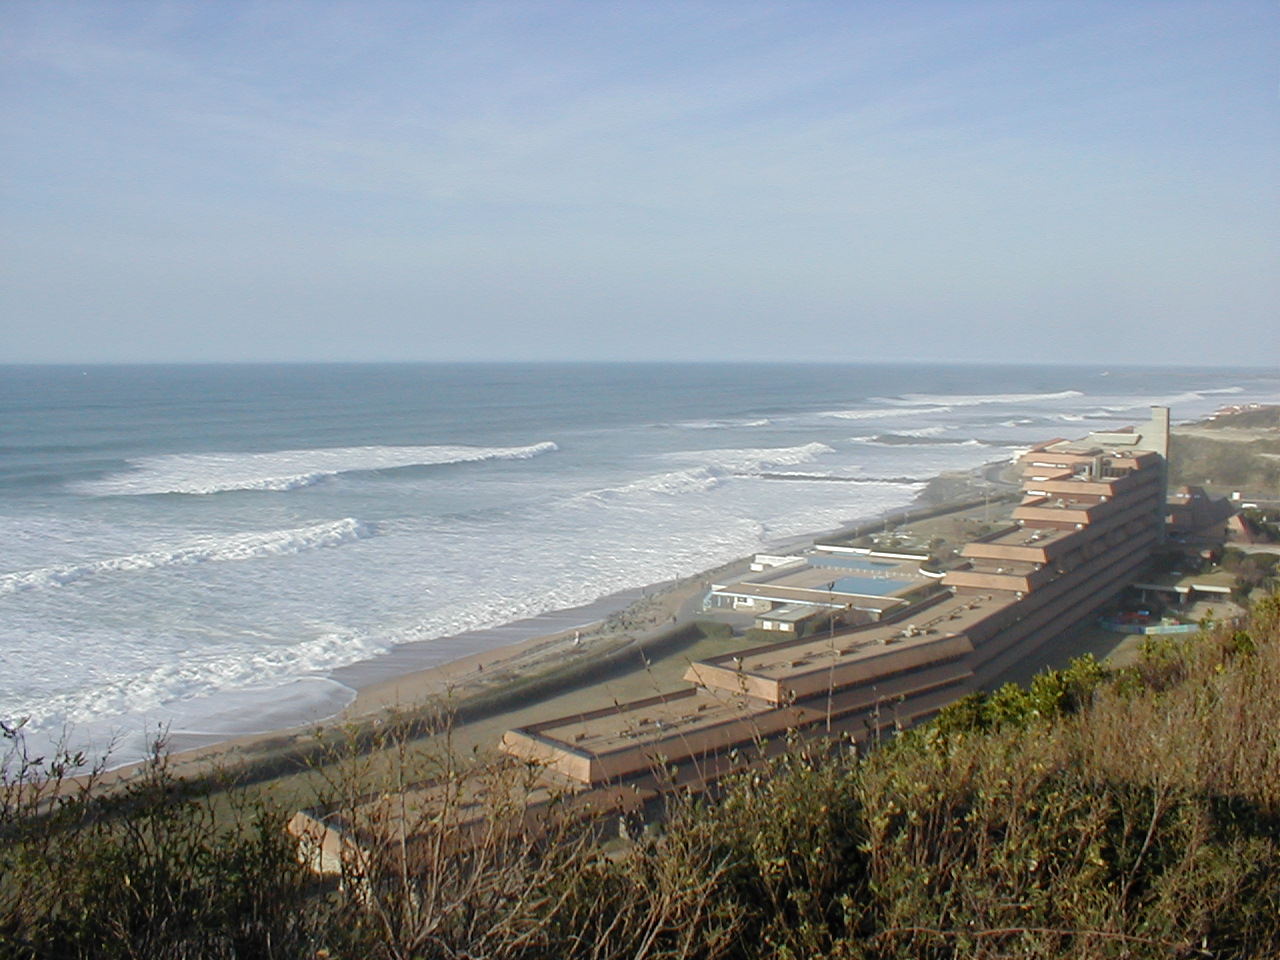
\includegraphics[width=.8\linewidth]{jfla.jpg}
  \caption{Les JFLA 2002, photographie par Maxence Guesdon}
  \label{fig:bienbelle}
\end{figure}

L'usage de~\texttt{includegraphics} avec une option~\texttt{width} permet une
utilisation facile d'images, comme illustré par la figure~\ref{fig:bienbelle}.

\subsection{Mathématiques}

Les environnements suivants ont été prédéfinis via le paquet~\texttt{amsthm}.

\begin{center}
  \begin{tabular}{lll}
    Environnement & Nom français & Nom anglais
    \\
    \hline
    \texttt{theo} & Théorème & \emph{Theorem}
    \\
    \texttt{prop} & Proposition & \emph{Proposition}
    \\
    \texttt{conj} & Conjecture & \emph{Conjecture}
    \\
    \texttt{coro} & Corollaire & \emph{Corollary}
    \\
    \texttt{lemm} & Lemme & \emph{Lemma}
    \\
    \texttt{defi} & Définition & \emph{Definition}
    \\
    \texttt{rema} & Remarque & \emph{Remark}
    \\
    \texttt{exem} & Exemple & \emph{Example}
  \end{tabular}
\end{center}

\subsection{Code source}

La classe~\texttt{jflart.cls} ne propose pas de paquet pour la coloration
syntaxique par défaut.
%
Les paquets~\texttt{listings} et~\texttt{minted} sont les plus fréquemment
utilisés.

% Pour utiliser le paquet~\texttt{listings}, il est recommandé de
% charger ce paquet en lui passant l'option~\texttt{final}~:
% \verb,\usepackage[final]{listings},. Ainsi, les extraits de code
% source seront bien affichés dans votre article, même lors de la
% production de la version soumise à relecture pour évaluation avec
% l'option~\texttt{review} de la classe \texttt{jflart.cls}.

\subsection{Bibliographie}

Vous pouvez au choix utiliser bibtex ou biblatex pour gérer votre bibliographie.
%
Merci d'utiliser le style de citation~\texttt{alpha-fr} avec bibtex, ou son
équivalent biblatex.

\subsection{Remerciements}

La classe ne propose pas d'environnement dédié pour les remerciements et sources de financement éventuelles.
%
Nous vous suggérons d'utiliser la commande~{paragraph\{Remerciements.\}} en
fin d'article.

\subsection{Autres ressources}

La classe~\texttt{jflart.cls} et sa documentation sont disponibles en
ligne~\cite{JFLART}.

\bibliographystyle{alpha-fr}
\bibliography{jflart}

\end{document}
